
The lecture today is about Partially Observable MDP (POMDP). The
main difference is that we will not observe the current state but
only a signal that depends on it.


\paragraph{Example:}\ \\
Assume we have four states, in linear order: $1,2,3,4$. We have an
action UP that with probability $0.90$ moves from $i$ to $i-1$ and
with probability $0.1$ moves to $i+1$. Similarly, we have an action
DOWN that with probability $0.90$ moves from $i$ to $i+1$ and with
probability $0.1$ moves to $i-1$. (In state $i=1$ if we need to move
to $i-1$ we stay in $i=1$ and in state $i=4$ if we need to move to
$i+1$ we stays in state $i=4$.)

One of the states, state $2$ has a reward, while the other states do
not have any reward. (See Figure~\ref{fig:Example-4states}.) The
only observation we see is the reward.

Initially, we know we are in a random state without a reward. This
implies that the distribution of where we are is $(1/3,0,1/3,1/3)$.
Assume we did an action UP and did not observe a reward. We now can
compute the posterior of our probability distribution.

First, we compute the state probability distribution, assuming any
current state.
\begin{enumerate}
\item
Assuming we are in state $i=1$, our state distribution will be
$(0.9,0.1,0,0)$.
\item
Assuming we are in state $i=2$, our state distribution will be
$(0.9,0,0.1,0)$.
\item
Assuming we are in state $i=3$, our state distribution will be
$(0,0.9,0,0.1)$.
\item
Assuming we are in state $i=4$, our state distribution will be
$(0,0,0.9,0.1)$.
\end{enumerate}

Since our prior state distribution was $(1/3,0/1/3,1/3)$ our
posterior state distribution (before observing the reward) is
$(0.3,1/3,0.3,1/15)$.

Given that we observed ``no reward'' we are not instate $2$ so the
posterior state distribution is $(0.45,0,0.45,0.1)$.


\begin{figure}
  % Requires \usepackage{graphicx}
  \begin{centering}
  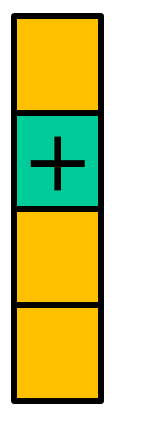
\includegraphics[width=0.1\textwidth]{Example-4states.PNG}\\
  \caption{The four state POMDP}\label{fig:Example-4states}
  \end{centering}
\end{figure}


\section{POMDP: model}

The model of a POMDP will be similar to that of an MDP with an
additional observation function. Namely,
\begin{itemize}
\item
$S$, a finite set of states.
\item
$A$, a finite set of actions.
\item
$p(s'|s,a)$, a probability distribution of next state given that we
are in state $s$ and do action $a$.
\item
$R(s,a)$ a random variable for the reward in state $s$ doing action
$a$, and $r(s,a)=E[R(s,a)]$.
\item
$q_0$ the initial state (can also be a distribution over states)
\item
$Ob$ is an observability distribution over $O$ a set of observable
signals. $O$ can be either finite of infinite. $Ob(o|s',a)$ is the
probability that we observe signal $o\in O$ if we reach state $s'$
after doing action $a$. (Note that in an MDP we have the observable
signals $O=S$ and $Ob(o|s',a)=s')$.
\end{itemize}

\subsection{Belief state}

The belief state tracks the state distribution, which captures our
current state. Each time we perform an action and observe an
observation we compute a new belief state, which is our posterior
distribution, given our action and observation.

The belief state is a sufficient statistics, implying that it has
all the information needed from the history. (Also, two histories
which reach the same belief state, we should behave identical for
them.)
%
Formally, a belief state $b$ is a distribution over states, i.e.,
$b\in[0,1]^{|S|}$ and $\sum_s b(s)=1$.

Given a belief state $b$ and an action $a$ and observation $o$, we
need to compute the next belief state $b'(s)=\Pr[s'|o,a,b]$. This
will be a deterministic function, and we will have
$b'=\calT(b,a,o)$.

\paragraph{Belief state computation:}\ \\
We compute the next belief state as follows:
\begin{align*}
b'(s') &= \Pr[s'|o,a,b]\\
&= \frac{\Pr[o|s',a,b]\Pr[s'|a,b]}{\Pr[o|a,b]}\\
&= \frac{\Pr[o|s',a]\sum_s \Pr[s'|a,b,s]\Pr[s|a,b]}{\Pr[o|a,b]}\\
&= \frac{Ob(o|s',a)\sum_s p(s'|a,s)b(s)}{\Pr[o|a,b]}
\end{align*}
where the first identity is the definition of the new belief state.
The second identity is Bayes rule. The third identity is adding a
conditioning over $s$. The last identity is translating the
probabilities to the POMDP parameters.

\paragraph{From POMDP to infinite MDP}\ \\
Consider the following MDP. The set of states are $B$ all the
possible belief states. (Note that $B$ is infinite!) The set of
actions is $A$ (finite). For each belief state $b$ and action $a$ we
define the expected reward $r(b,a)=\sum_s b(s)r(s,a)$. The
transition probability is to move to $b'=\calT(b,a,o)$ and is
deterministic. (Namely, $\Pr[b'=\calT(b,a,o)|b,a,o]=1$ and
$\Pr[b'\neq \calT(b,a,o)|b,a,o]=0$.)


\section{Value function}
The value function will be mapping belief states to expected return.
The return can be any of the return we discussed: finite horizon,
discounted, of average reward.

We would like to characterize the optimal value function. For a
finite horizon it will be piece-wise linear and convex. (For
discounted it will be convex.) Our algorithmic challenge is to
handle the infinite state spaces. We will concentrate on the case of
finite horizon.

For simplicity, we start with a horizon of length $H=1$. Namely, we
would like to maximize our immediate reward. For each action, our
immediate reward is a linear function in the belief state. Namely,
$r(b,a)=\sum_s b(s)r(s,a)$. The optimal action for $H=1$ is the
action $a$ that maximizes the expected reward. Namely,
$V^*_1(b)=\max_a r(b,a)=\max_a [\sum_s b(s)r(s,a)]$. This implies
that the optimal value function is a maximum of linear functions.
This gives us a finite representations. It also partitions the space
of belief states to regions, which in each region there is an
optimal action. The partition to the regions is done by intersecting
hyper-planes. The region in which $a_1$ is the best action is define
by $\{b: \forall a\neq a_1 \sum_s b(s)r(s,a_1)\geq \sum_s
b(s)r(s,a)\}$.

We will now consider a horizon of $H=2$. We will partition the task
to three steps. In the first step, we will assume that we are in
belief state $b$ perform action $a_1$ and observe $o_1$. In the
second step, we assume we are in belief state $b$ and perform action
$a_1$. In the third step, we only assume we are in belief state $b$.

Assume we  we are in belief state $b$ perform action $a_1$ and
observe $o_1$. We would like to compute $V_H(b|a_1,o_1)$ for $H=2$.
For the first step, given that we do action $a_1$, we can compute
the expected immediate reward $\sum_s b(s)r(s,a_1)$. Now, we move
from belief state $b$ to belief state $b'=\calT(b,a_1,o_1)$. When we
reach $b'$ we have only one step remaining, so we perform the best
action and get $V^*_1(b')$. This implies that
$V^*_2(b|a_1,o_1)=r(b,a_1)+V^*_1(b')$. (See
Figure~\ref{fig:belief-state-1}.) This implies that
$V^*_2(b|a_1,o_1)$ is piece-wise linear.

\begin{figure}
  % Requires \usepackage{graphicx}
  \begin{centering}
  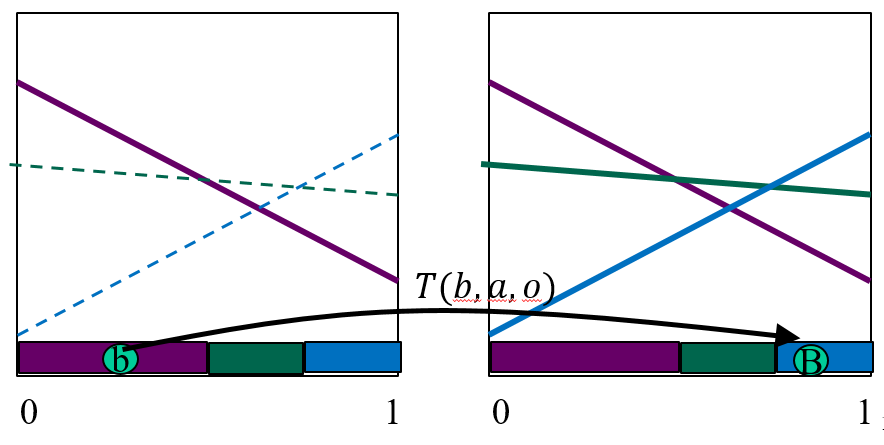
\includegraphics[width=0.5\textwidth]{belief-state-1.PNG}\\
  \caption{Computing $V^*_2(b|a_1,o_1)$}\label{fig:belief-state-1}
  \end{centering}
\end{figure}

We can now do the same for each possible observations (assume the
set of observations is finite, for simplicity). This implies that we
have the values of $V^*_2(b|a_1,o)$ for any $o\in O$. This allows us
to compute $V^*_2(b|a_1)$, by simply averaging over the
observations. $V^*_2(b|a_1)=\sum_o V^*_2(b|a_1,o)\Pr[o|b,a_1]$. We
can compute $\Pr[o|b,a]=\sum_{s,s'} b(s)p(s'|s,a)Ob(o|s',a)$.

Given that we can compute $V_2^*(b|a)$ for any action $a\in A$, we
can deduce $V_2^*(b)=\max_a V_2^*(b|a)$.

We can now compute for a longer horizon, say $H=3$, using dynamic
programming. We want to compute $V^*_3(b)$. We first compute the
function $V_2^*(\cdot)$. For each action $a_i$ and observation $o_j$
we compute $V^*_3(b|a_i,o_j)$. This is done by first computing
$r(b,a_i)$ and $b'=\calT(b,a_i,o_j)$. Then we compute
$V^*_3(b|a_i,o_j) = r(b,a_i)+V^*_2(b')$.

\paragraph{Optimal value function}\ \\
For the finite horizon the optimal value function $V^*_H(b)$ is
define as follows,
\[
V^*_H(b)=\max_a [r(b,a)+\sum_o \Pr[o|b,a]V^*_{H-1}(\calT(b,a,o))]
\]
and the optimal policy is
\[
\pi_H^*(b)=\arg\max_a [r(b,a)+\sum_o
\Pr[o|b,a]V^*_{H-1}(\calT(b,a,o))]
\]

\begin{theorem}
For the finite horizon, the function $V^*_H$ is piece-wise linear
and convex. In addition, there exists a collection of
$\Theta=\{\theta_i\in \mathbb{R}^{|S|}\}$ such that
$V^*_H(b)=\max_{\theta_i\in\Theta} \sum_s b(s)\theta_i(s)$.
\end{theorem}


\begin{proof}
The proof is by induction on the horizon. For the base case, $T=1$,
we have $V^*_1(b)=\max_a b^\top r(\cdot,a)$.

For the inductive step, assume that for $i-1$ we have a set
$\Theta_{i-1}$, such that $V^*_{i-1}(b_{i-1})=\max_{\theta\in\Theta_{i-1}}
b_{i-1}^\top \theta$.

Consider belief state $b_i$, and assume that after action $a$ and
observed $o$ we reach belief state $b^{a,o}_{i-1}$, i.e. $b^{a,o}_{i-1}(s'|b_i,a,o)=\Pr[s',a,o]$. For
$V^*_i(b_i)$ we have
\begin{align*}
V^*_i(b_i)=&\max_a (r(b_i,a)+\sum_o \Pr[o|b_i,a]V^*_{i-1}(\calT(b_i,a,o)))\\
=&\max_a (r(b_i,a)+\sum_o
\Pr[o|b_i,a]\max_{\theta\in\Theta_{i-1}}\theta^\top b_{i-1}^{a,o})
\end{align*}
where the second identity follows from the inductive assumption.

We will now concentrate on part of the inner sum in the expression:
\begin{align*}
\sum_o \Pr[o|b_i,a]\max_{\theta\in\Theta_{i-1}}\theta^\top b_{i-1}^{a,o}) =&
\sum_o \max_{\theta\in\Theta_{i-1}} \Pr[o|b_i,a]
\theta^\top b_{i-1}^{a,o})\\
=& \sum_o \max_{\theta\in\Theta_{i-1}} \Pr[o|b_i,a]
\sum_{s'}\Pr[s'|b_i,a,o]\theta(s')\\
=& \sum_o \max_{\theta\in\Theta_{i-1}} \sum_{s'} \Pr[s',o|b_i,a] \theta(s')\\
=& \sum_o \max_{\theta\in\Theta_{i-1}} \sum_s b_i(s) \left[\sum_{s'} \Pr[s',o|s,a] \theta(s')\right]\\
\end{align*}
where the second identity writes the belief state $b_{i-1}^{a,o}$ explicitly;
the third identity uses the fact that $\Pr[X]\Pr[Y|X]=\Pr[X,Y]$;
the last identity marginalizes over $b_i$.

Returning to $V^*_i(b_i)$.
%Let $\Theta_i=\cup_a \Theta^{a}_{i-1}
\begin{align*}
V^*_i(b_i)=&\max_a (r(b_i,a)+\sum_o \Pr[o|b_i,a]V^*_{i-1}(\calT(b_i,a,o)))\\
=&\max_a  (r(b_i,a)+\sum_o \max_{\theta^{a,o}\in\Theta_{i-1}}  \sum_s b_i(s)\sum_{s',o} \Pr[s',o|s,a]\theta^{a,o}(s'))\\
=&\max_{(\theta^{a,o})_{o\in O,a\in A}\in\Theta^a_{i-1}} \max_a (\sum_s b_i(s)(r(s,a)+\sum_{s',o} \Pr[s',o|s,a]\theta^{a,o}(s')))\\
=&\max_{\theta\in \Theta_i} b_i^\top \theta
\end{align*}
where the second identity is from the previous derivation;
the third identity follows by maximizing over each action $a$ and observation $o$ seperately;
and the last idetity follows for
\[
\Theta_i=\{\theta: \exists a\in A, \theta^{a,o}\in\Theta_{i-1} :\theta(s)=r(s,a)+\sum_{s',o}
\Pr[s',o|s,a]\theta^{a,o}(s') \}.
\]
Note that for each action $a\in A$ we have a vector $\theta^{a,o}$ for any possible observation $o\in O$.
\end{proof}


For the discounted setting we have
\[
V^*(b)=[r(b,a)+\gamma\sum_o \Pr[o|b,a]V^*_{H-1}(\calT(b,a,o))]
\]

%\bigskip

One can also show the following.
\begin{theorem}
For the discounted return, the function $V^*$ is convex.
\end{theorem}

\paragraph{Policy Tree}\ \\
How does the optimal finite horizon policy can be implemented. We
can create a tree. In each node of the tree, we can label it by the
action we perform. We label the outgoing edges by the observation we
receive. We start at the root. The action at the root is the action
we perform at the initial state. Given the observation we receive,
we continue to the next node in the tree. The label of that node is
the action we perform and so on. The depth of the tree is $H$ for a
finite horizon of length $H$.

\subsection{Value Iteration}

We can run a value iteration in the POMDP (actually, on the belief
states. We can write the update as follows:
\begin{align*}
V^{a,o}_{t}(b)=&\frac{r(b,a)}{|O|}+\gamma\Pr[o|b,a]V_t(\calT(b,a,o))\\
V_{t}^a(b)=&\sum_o V^{a,o}_{t}(b)\\
V_{t+1}^*(b)=&\max_a V_{t}^a(b)\\
V_{t+1}^*(b) =& \max_a [r(b,a)+\gamma\sum_o V_t^*(\calT(b,a,o)
\end{align*}
%\begin{align*}
%V_{t+1}^*(b) =& \max_a [r(b,a)+\gamma\sum_o V_t^*(\calT(b,a,o)\\
%V_{t+1}^*(b)=&\max_a V_{t}^a(b)\\
%V_{t}^a(b)=&\sum_o V^{a,o}_{t}(b)\\
%V^{a,o}_{t}(b)=&\frac{r(b,a)}{|O|}+\gamma\Pr[o|b,a]V_t(\calT(b,a,o))
%\end{align*}

Assume that $V_t$ is piece-wise linear. Namely, there exists a set
$\Theta_t$ such that
\[
V_t(b)=\max_{\theta\in\Theta_t}\theta^\top b
\]
For $V_t^{a,o}$ we have that $b'=\calT(b,a,o)$ is linear in $b$,
i.e., there is a matrix $M$ such that $b'=Mb$. (Note that $M$
depends on $a$ and $o$.) The value of $V_t^{a,o}$ is
\[
V_t^{a,o}(b')=\max_{\theta\in\Theta_t} b^\top \frac{r(b,a)}{|O|}+
\theta^\top b'= \max_{\theta\in\Theta_t} b^\top (\theta
M+\frac{r(b,a)}{|O|})
\]
This implies that we can define $\Theta_t^{a,o}=\{\theta^\top
M:\theta \in \Theta_t\}$.

For $V^a_t$ we have that
\[
V_t^a(b)=\sum_o V_t^{a,o}(b)=\sum_o \max_{\theta\in\Theta_t^{a,o}}
\theta^\top b=\max_{\theta\in\Theta_t^{a}}\sum_o  \theta^\top b
\]
where
\[
\Theta^a_t=\{\sum_o
\theta^{a,o}|\theta^{a,o}\in\Theta^{a,o}_t\}
\]

For $V_{t+1}^*$ we have
\[
V^*_{t+1}(b)=\max_a V_t^a(b)=\max_{\theta\in\Theta_{t+1}}
\theta^\top b
\]
where $\theta_{t+1}=\cup_a \Theta^a_t$.
%

The complexity of value iteration depends on $\Theta_t$. For each
action $a$ and observation $o$ we have $|\Theta^{a,o}_t|\leq
|\Theta_t|$. For each action $a$ we have $|\Theta^a_t|\leq
{|\Theta^{a,o}_t|}^{|O|}\leq {|\Theta_t|}^{|O|}$. For $\Theta_{t+1}$
we have $|\Theta_{t+1}|\leq \sum_a |\Theta_t^a|\leq |A|\cdot
|\Theta_t|^{|O|}$.

The complexity is exponential in $|O|$ in each iteration! Pruning
can help, but the exponential time seems unavoidable.

\subsection{Hardness}

Many computational problems related to POMDPs are hard. For the
finite horizon, even with a unique start state, it is P-SPACE
complete to compute the return of the optimal policy.

For the finite horizon, in the case that there are no observations,
it is NP complete to compute the return of the optimal policy. (We
will show this simple hardness result.)

Assume we have no observations. This implies that we need to compute
a sequence of $H$ actions. The optimal policy will be the sequence
of $H$ actions that will maximize the return. We will show a
reduction to SAT.

Given a SAT formula over $n$ variables we create the following
POMDP. For each clause we create the following POMDP gadget. We have
always two actions $0$ and $1$. We create two lines of length $n$,
one line ends in a state with reward $1$ and the other in a state
with reward $0$. All other rewards will be zero. We ``think'' of the
state in the line as a number in $[1,n]$ and we associate the state
$i$ it with the variable $x_i$.

We start at the line ending with $0$. All the transition of states
in the line ending in $1$ simply continue to the next state, i.e.,
from $i$ to $i+1$ (for both actions). For the line ending in zero,
for each state $i$ where $x_i$ nor $\bar{x}_i$ do not appear in the
clause, we continue to the next state on this line, with both
actions.

For state $i$ in the line that ends in $0$, if $x_i$ appears
 in the clause, then in state $s_i$ with action $1$ we
move to the $i+1$ state in the line ending in $1$, and with action
$0$ we move to state $i+1$ in the line ending in zero.
%
Similarly, if $\bar{x}_i$ appears in the clause,  then in state
$s_i$ with action $0$ we move to the $i+1$ state in the line ending
in $1$, and with action $1$ we move to state $i+1$ in the line
ending in zero.

It is not hard to see that the sequence of $n$ actions will lead to
the reward $1$ if and only if it represents an satisfying assignment
to the clause.

We now take the gadgets for all the clauses, and select our initial
state to uniformly at random to be the start state of one of the
gadget (which represent a clause).

If the SAT formula is satisfiable, there is an assignment that
satisfies all the clauses. Therefore guarantees a return of $1$.

Otherwise for each sequence of action, which represent an
assignment, there is some clause which is not satisfied. This
implies that the return is at most $1-1/m$, where $m$ is the number
of clause.

\paragraph{Remark:} Actually, we can get from the same reduction
also a hardness to approximate result. We simply consider the
MAX-SAT problem. For 3-SAT it is NP-hard to decide distinguish
between satisfying $7/8+\epsilon$ of the terms or all the terms.
This implies that it is NP-hard to distinguish between a return of
$7.8+\epsilon$ or $1$.

\subsection{Policy Plan: Automata}

A simple class to describe the policy is a finite automata with
output, which is called a Moore automata. The outputs will be the
selected actions and the inputs are the observations. While it is
true that this class of policies is not universal, namely, not any
policy can be represented in this way, many policies can be.

One nice observation regarding this class of polices is that we can
efficiently compute the value function of a given automata. Assume
that $\pi$ is described by an automata. The value of $\pi$ from
state $s$ when its automata is in state $\sigma$ is
\[
V^\pi(s;\sigma)=r(s,a)+\gamma \sum_{o,s'}
p(s'|s,a)Ob(o|s'a)V^\pi(s';\sigma')
\]
where $a=\pi(\sigma,o)$ the action selected by $\pi$ when in state
$\sigma$ of the automata and observes $o$, and $\sigma'$ is the next
state in the automata, given we are in state $\sigma$ and observe
$o$.

This implies that we have a set of linear equations and we can solve
them efficiently!


\section{Reusable trajectories}

Our goal is given a set of deterministic policies $\Pi$, to estimate
for each $\pi\in \Pi$ the value $V^\pi(s_0)$, its expected return.
We want a set of trajectories that would be relatively small
compared to $\Pi$, hopefully logarithmic in $|\Pi|$.

We will generate a set of trajectories $\Gamma$ in the following
simple way. We use a completely random policy to select the actions.
Namely, $\pi_R(a|b)=1/|A|$. We generate $m$ such trajectories.

We estimate the return of a policy $\pi\in \Pi$ in the following
way. Let $\Gamma_\pi$ all the trajectories that agree with $\pi$.
(Recall, $\pi$ is deterministic.) We set
\[
\hat{V}^\pi(s_0)=\frac{1}{|\Gamma_\pi|}\sum_{h\in \gamma_\pi}
return(h)
\]

The main issue will be: how large $m$ has to be, in order to
guarantee with probability $1-\delta$ that the error for any $\pi\in
\Pi$ in the estimation will be at most $\epsilon$. We will look at
$m$ as a function of the error $\epsilon$, the confidence $\delta$,
the number of policies $|\Pi|$, and the maximum return $V_{max}$.

The proof follows in the following steps. Let $acc_\pi(h)=1$ if
$\pi$ agrees on all the actions in $h$. The following lemma states
that for any policy, the probability that it agrees with the
trajectory of length $H$ is exactly $1/|A|^H$.
\begin{lemma}
For a finite horizon $H$, for any policy $\pi$ we have
$\Pr_h[acc_\pi(h)=1]=\frac{1}{|A|^H}$.
\end{lemma}

Let $D_\pi$ be the distribution over histories generated by policy
$\pi$. The following lemma states that the distribution of the
random policy, condition of policy $\pi$ agreeing with the actions,
is identical to that of generated by policy $\pi$.
\begin{lemma}
\[
D_\pi(h)=D_{\pi_R}(h|acc_\pi(h)=1)
\]
\end{lemma}

The following lemma states that with high probability, for every
$\pi\in \Pi$ we have that the size of $|\Gamma_\pi|$ is exponential
in the horizon.
\begin{lemma}
For
\[
m> 8|A|^{H}\frac{V^2_{max}}{\epsilon^2}\log(2|\Pi|/\delta)
\]
with probability $1-\delta/2$ for every $\pi\in \Pi$ we have
\[
|\Gamma_\pi|\geq \frac{m}{2^{H+1}}>
4\frac{V^2_{max}}{\epsilon^2}\log(2|\Pi|/\delta)
\]
\end{lemma}

The following lemma states that if every $\Gamma_\pi$ is of
sufficient size, then for each policy $\pi$ we have a good
approximation.
\begin{lemma}
If for every $\pi\in \Pi$ we have
\[
|\Gamma_\pi|\geq \frac{m}{2|A|^{H}}> 4
\frac{V^2_{max}}{\epsilon^2}\log(2|\Pi|/\delta)
\]
then with probability $1-\delta/2$, for every $\pi\in \Pi$ we have
\[
|\hat{V}^\pi (s_0)-V^\pi(s_0)|\leq \epsilon
\]
\end{lemma}


The theorem concludes and establishes the sample size for a PAC
guarantee.
\begin{theorem}
For
\[
m> 8|A|^{H}\frac{V^2_{max}}{\epsilon^2}\log(2|\Pi|/\delta)
\]
with probability $1-\delta$, for every $\pi\in \Pi$ we have
\[
|\hat{V}^\pi (s_0)-V^\pi(s_0)|\leq \epsilon
\]
\end{theorem}



















%
